\documentclass[11pt,a4paper]{article}
\usepackage[margin=1in]{geometry}
\usepackage{array}
\usepackage{graphicx}
\usepackage{caption}
\usepackage{CJKutf8}

\begin{document}
\begin{CJK}{UTF8}{bsmi}

\section*{Sample PDF for IDP Routing (OCR vs VLM)}

\subsection*{Page 1: Clean Text (expect OCR)}
這是一份用來驗收 IDP 流水線的測試文件。目標是讓系統在 \textbf{auto} 路由下，
能依據 OCR 品質評分決定是否 fallback 到 VLM。

English snippet: The quick brown fox jumps over the lazy dog.
關鍵字：Qdrant / Neo4j / GraphRAG / lineage / route\_trace

\newpage
\subsection*{Page 2: Table (may trigger fallback)}
\begin{table}[h]
\centering
\caption{Monthly KPI Table}
\begin{tabular}{|c|c|c|c|c|}
\hline
Month & Users & Revenue(NTD) & ErrorRate(\%) & Note \\
\hline
Jan & 1200 & 350000 & 1.2 & stable \\
Feb & 1800 & 420000 & 2.8 & peak load \\
Mar & 900 & 210000 & 0.9 & recovery \\
Apr & 1600 & 390000 & 3.5 & throttling \\
May & 2000 & 510000 & 4.1 & overload \\
\hline
\end{tabular}
\end{table}

\newpage
\subsection*{Page 3: Chart Image + Text (often best for VLM)}
(請你把一張圖命名為 \texttt{chart.png} 放在同資料夾，這頁就會內嵌圖表。)
\begin{figure}[h]
\centering
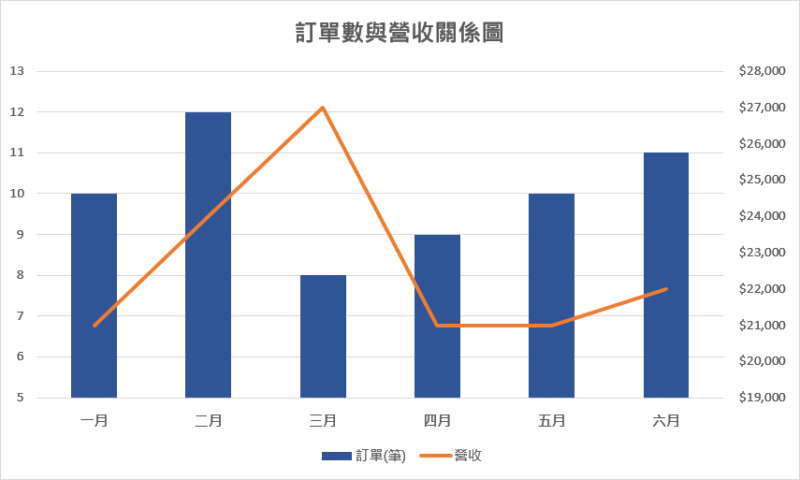
\includegraphics[width=0.9\linewidth]{chart.png}
\caption{Simple chart for routing test}
\end{figure}

圖表重點：四月與五月 ErrorRate 明顯上升，可能與上游模型服務過載相關。

\newpage
\subsection*{Page 4: Scan-like (text as image)}
這一頁建議你用截圖方式把一段文字做成圖片，再命名為 \texttt{scan.png} 放進來：
\begin{figure}[h]
\centering
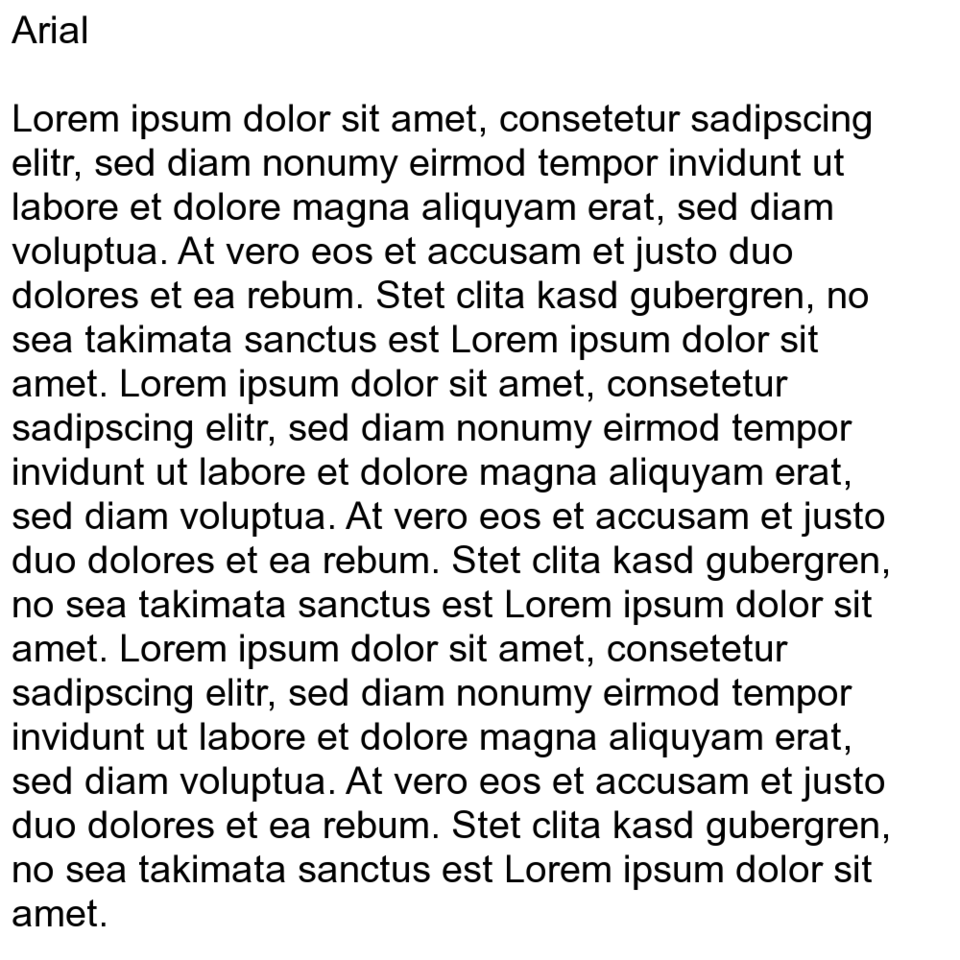
\includegraphics[width=0.9\linewidth]{scan.png}
\caption{Scan-like page to stress OCR}
\end{figure}

\end{CJK}
\end{document}